\documentclass[12pt,a4paper,titlepage]{article}

\usepackage{preamble}

\title{Représentation  Temps-Fréquence : travaux pratiques}
\author{Yassine Jamoud, Samy Haffoudhi}
\date{\today}

\begin{document}

\maketitle

\setcounter{section}{1}

\section{Représentation temps-fréquence de signaux simulés}

\subsection{Génération de signaux}

Représentons l'allure temporelle, la phase instantanée et la fréquence instantanée des signaux
mono-composantes $x_1$ et $x_2$ :

\begin{figure}[H]
    \caption{allure temporelle, phase et fréquence instantanée de $x_1$ et $x_2$}
    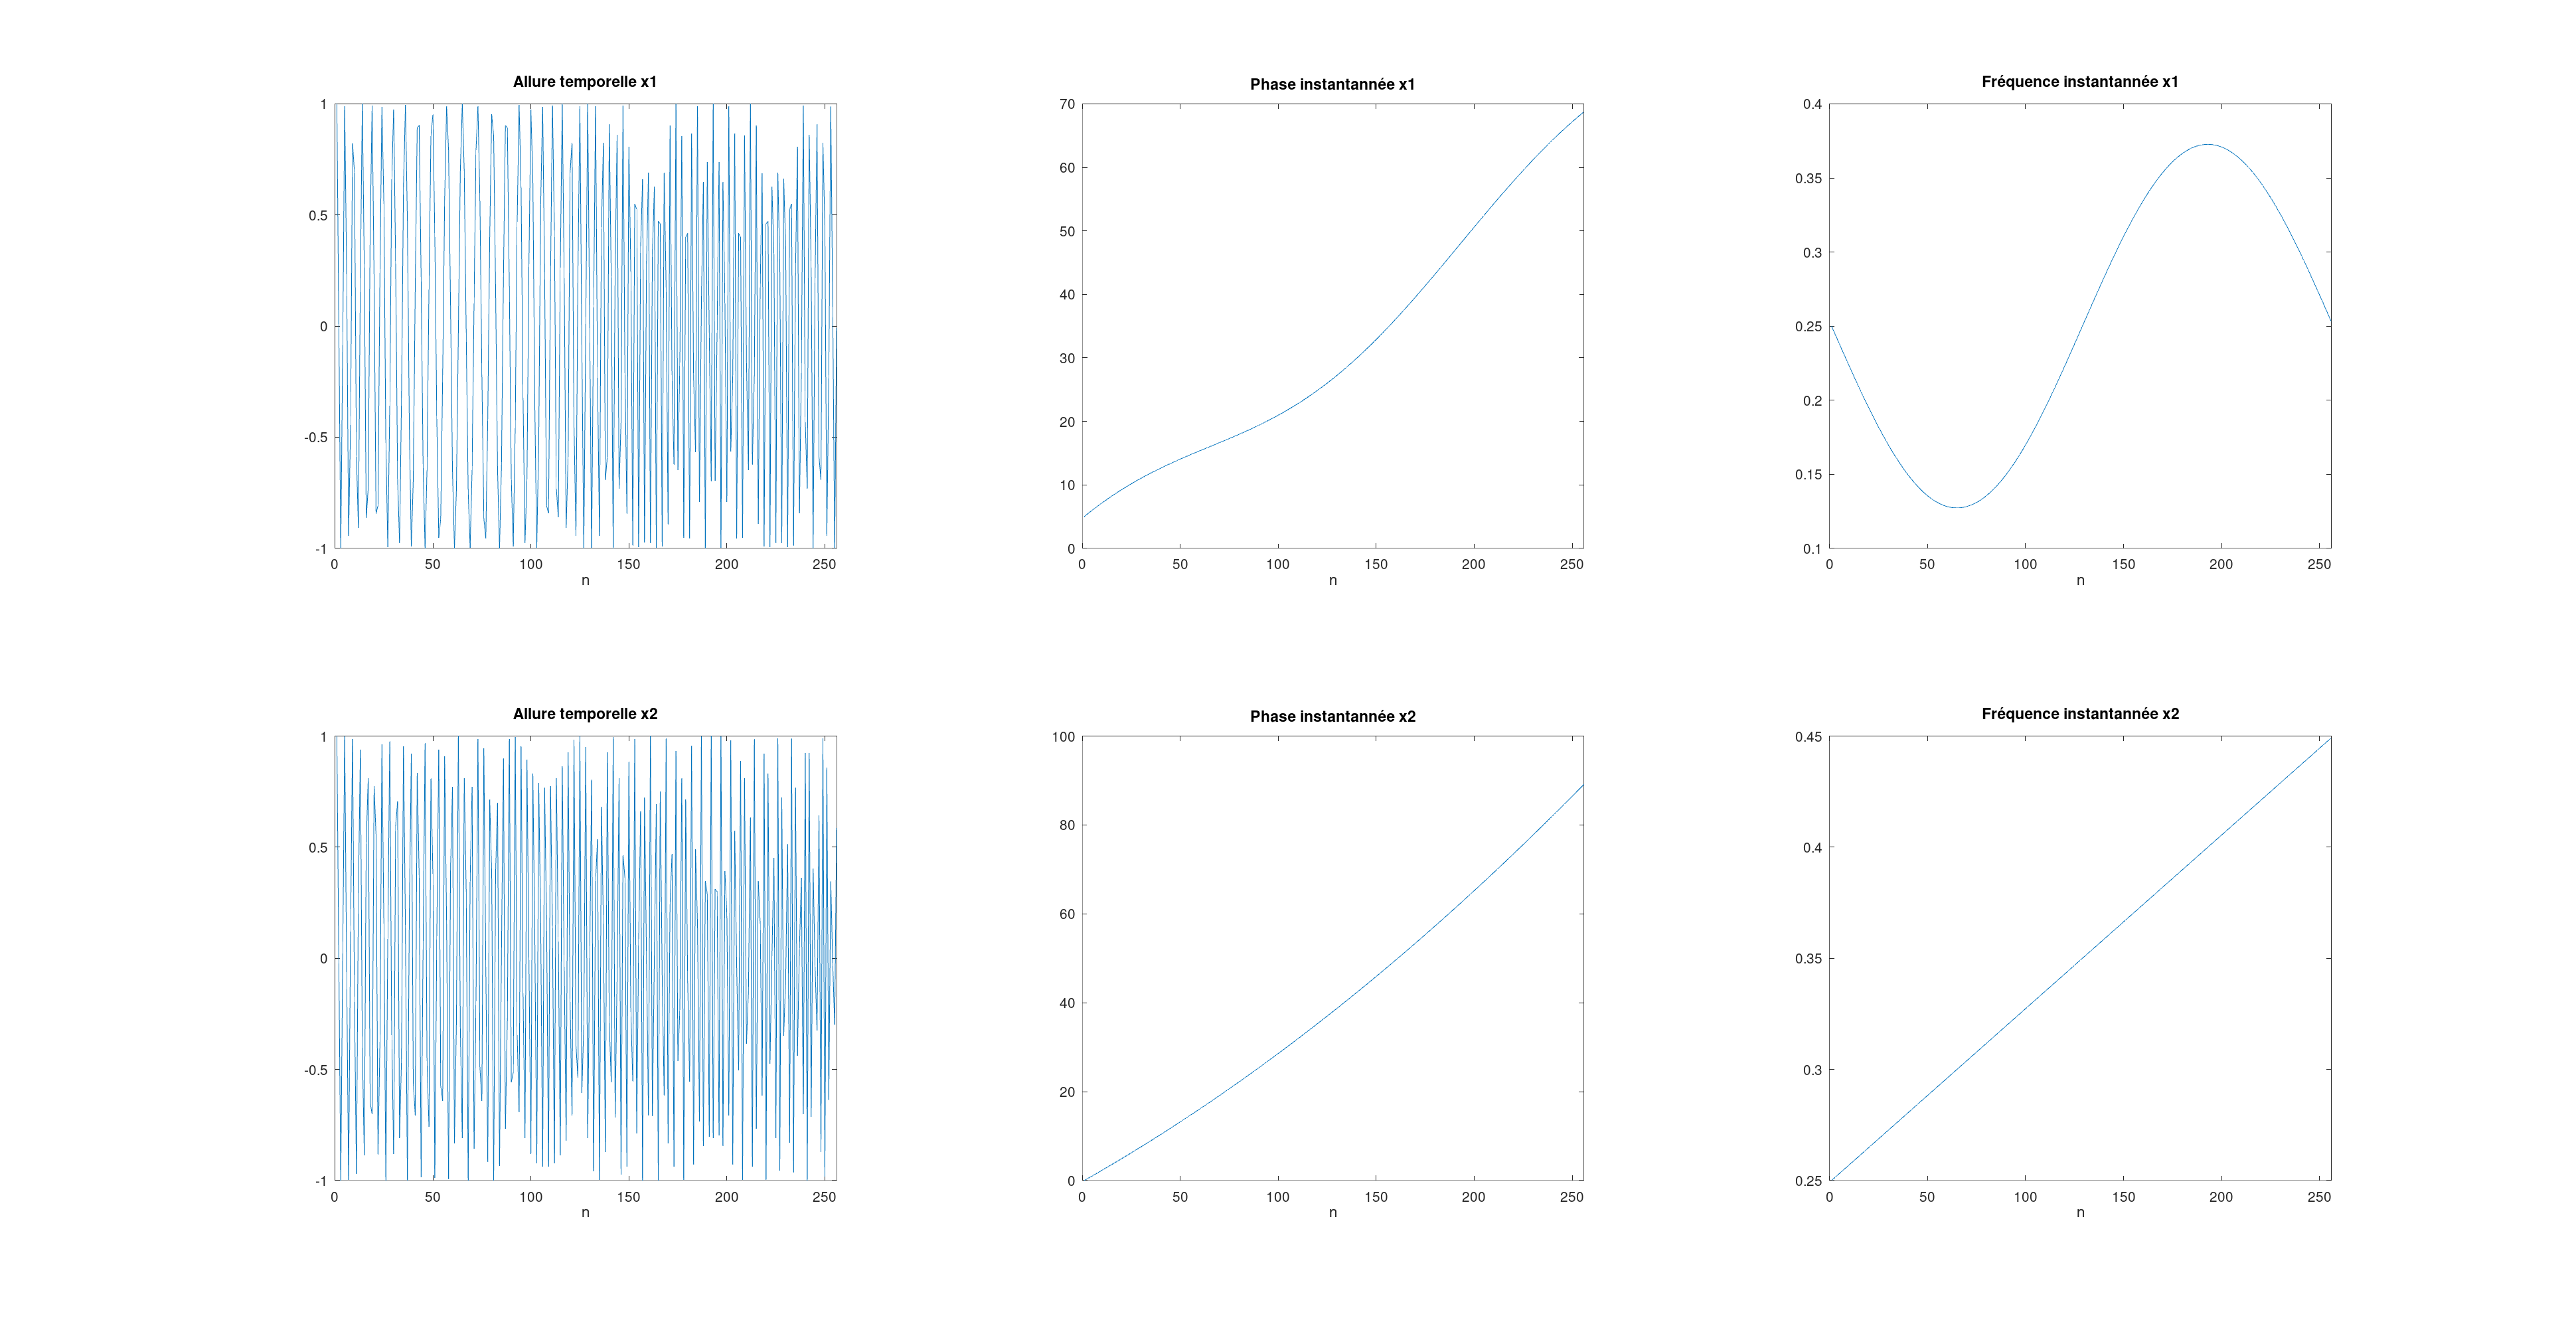
\includegraphics[width=\textwidth]{ex1q1}
    \centering
\end{figure}

Représentons maintenant l'allure du signal $x_3$, somme de quatre atomes gaussiens :

\begin{figure}[H]
    \caption{Allure temporelle du signal $x_3$}
    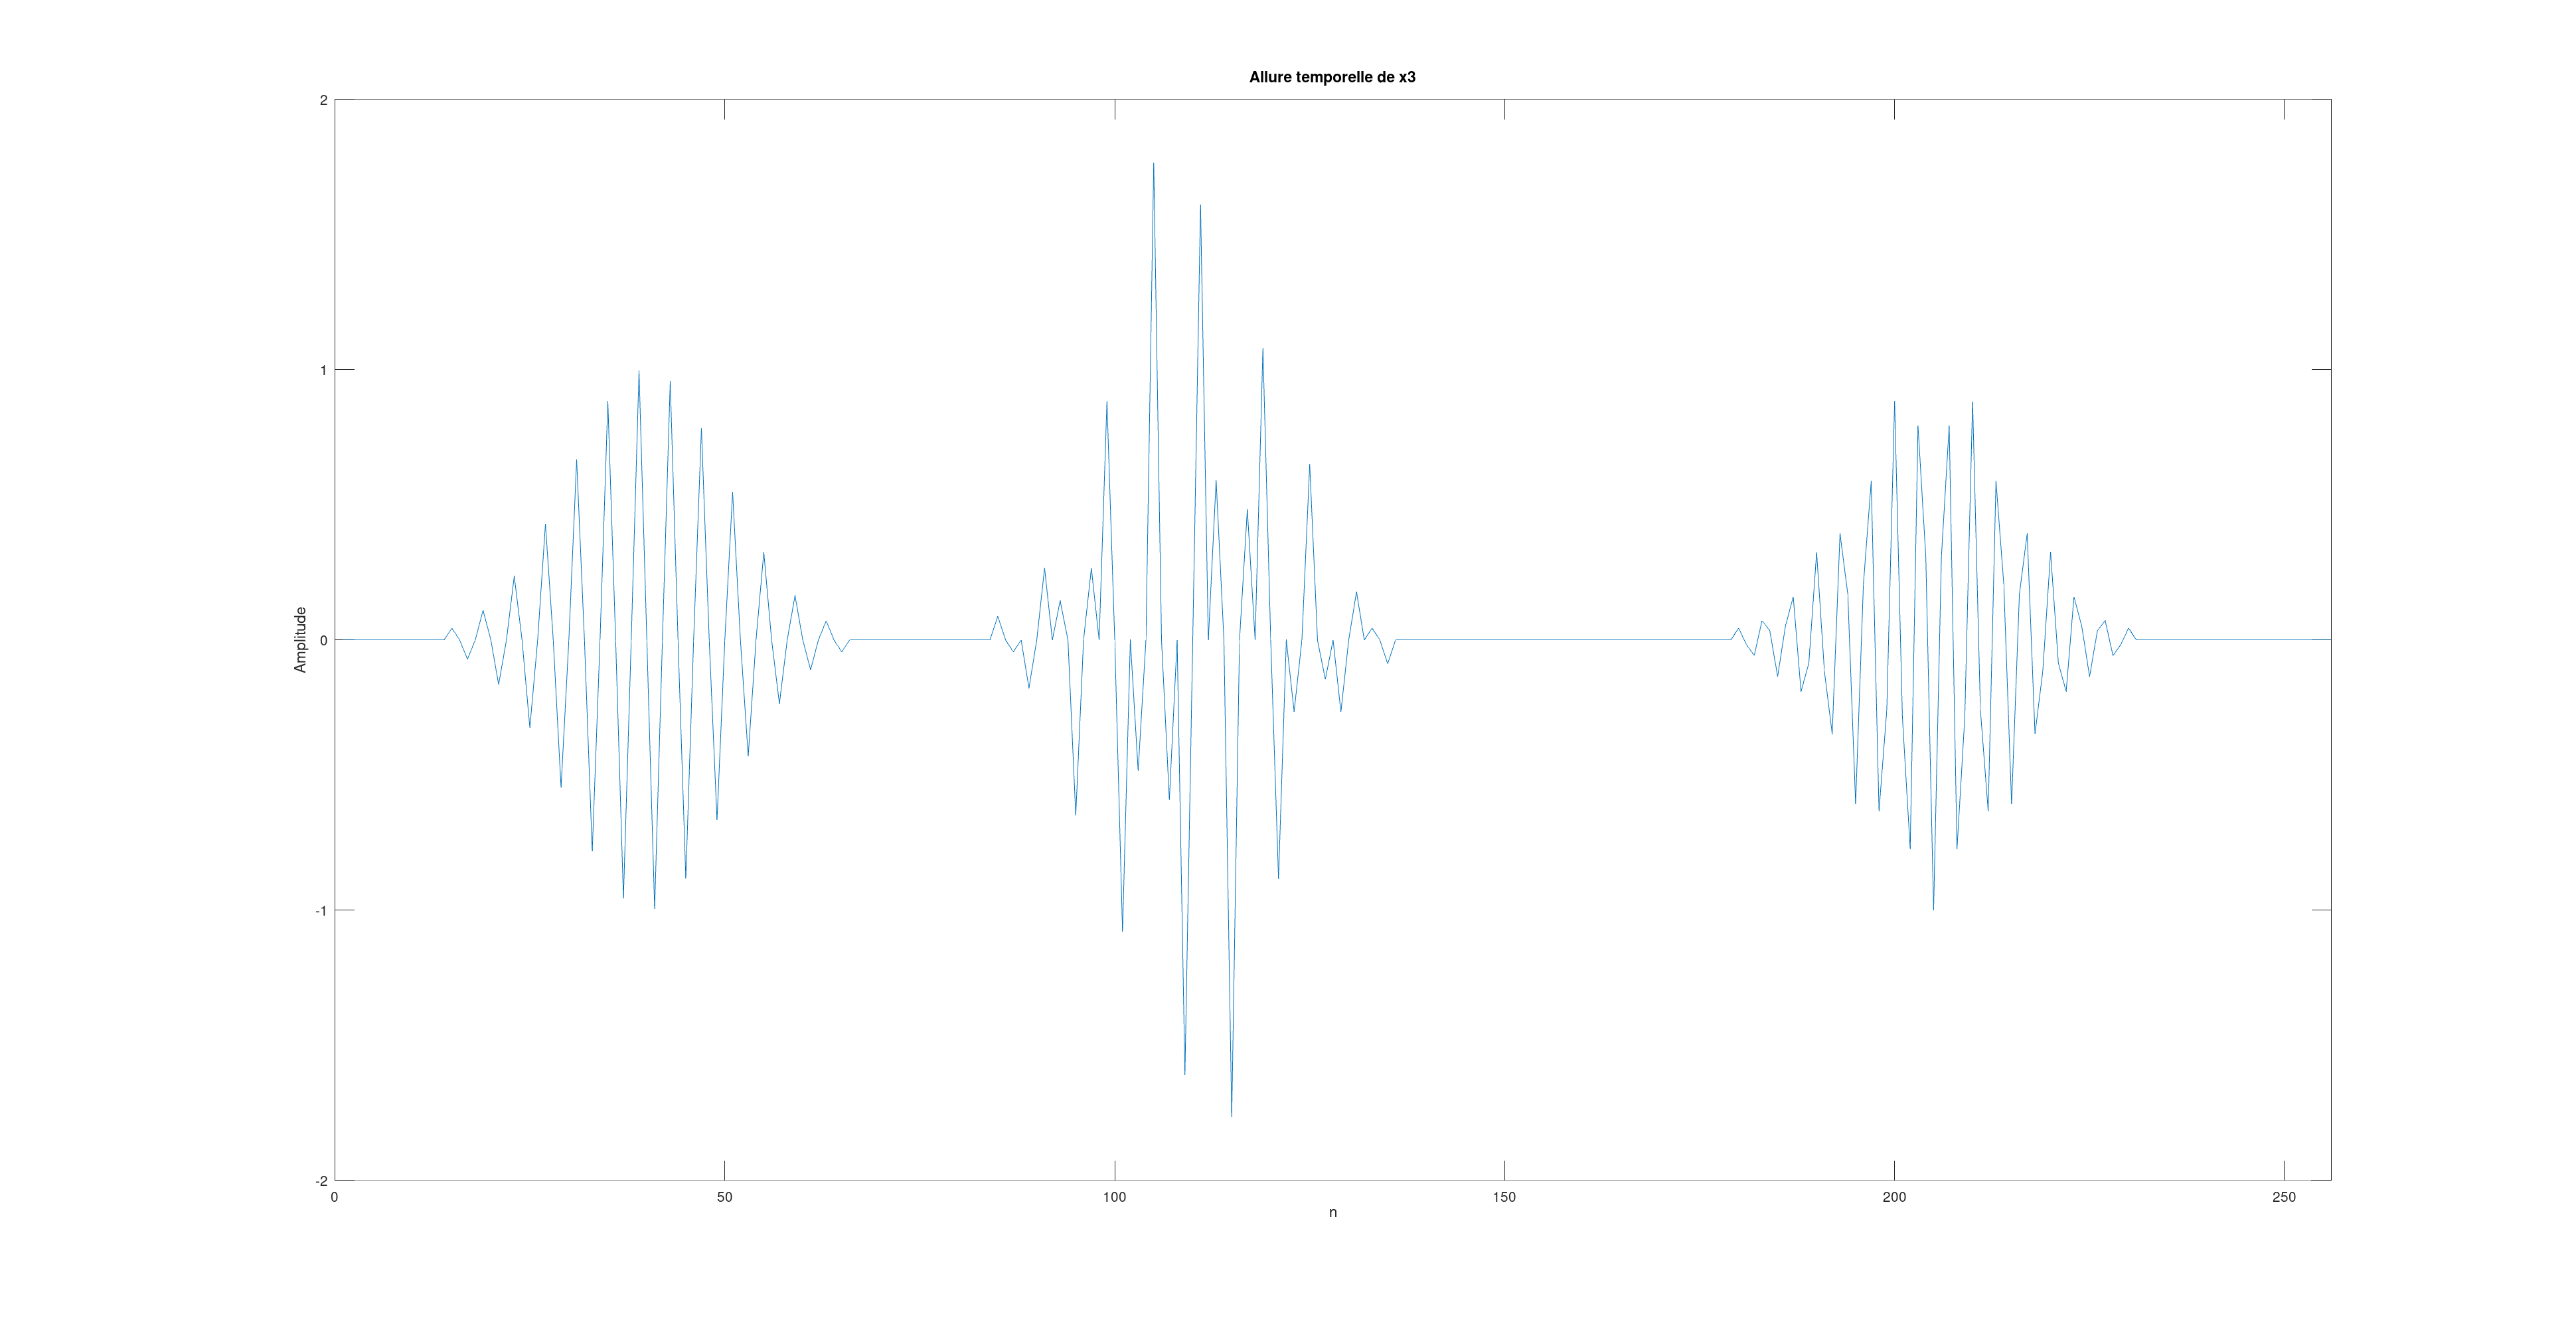
\includegraphics[width=\textwidth]{ex1q2}
    \centering
\end{figure}

Nous avons obtenus ces différentes figures à l'aide du script présenté en \textbf{Annexe A} et par le calcul
au préalable de $f_i(t) = \frac{d\phi_i(t)}{dt}$.

\subsection{Représentation temps-fréqyence}

Pour chaque signal nous allons maintenant représenter :

\begin{itemize}
    \item{Le spectrogramme en utilisant une fenêtre de Hamming de longueur \texttt{Nh} = 17, 33, 65
        et 129.}
    \item{La transformée de Wigner-Ville}
    \item{La transformée de pseudo-Wigner-Ville en utilisant une fenêtre de Kaiser avec \texttt{Nh}
        = 63.}
    \item{La transformée de pseudo-Wigner-Ville lissée avec des fenêtres de Kaiser de longueur
        \texttt{Ng} = 33 et \texttt{Nh} = 63, puis \texttt{Ng} = 15 et \texttt{Nh} = 63.}
\end{itemize}

On obtient les figures suivantes :

\begin{figure}[H]
    \caption{Tracés $x_1$}
    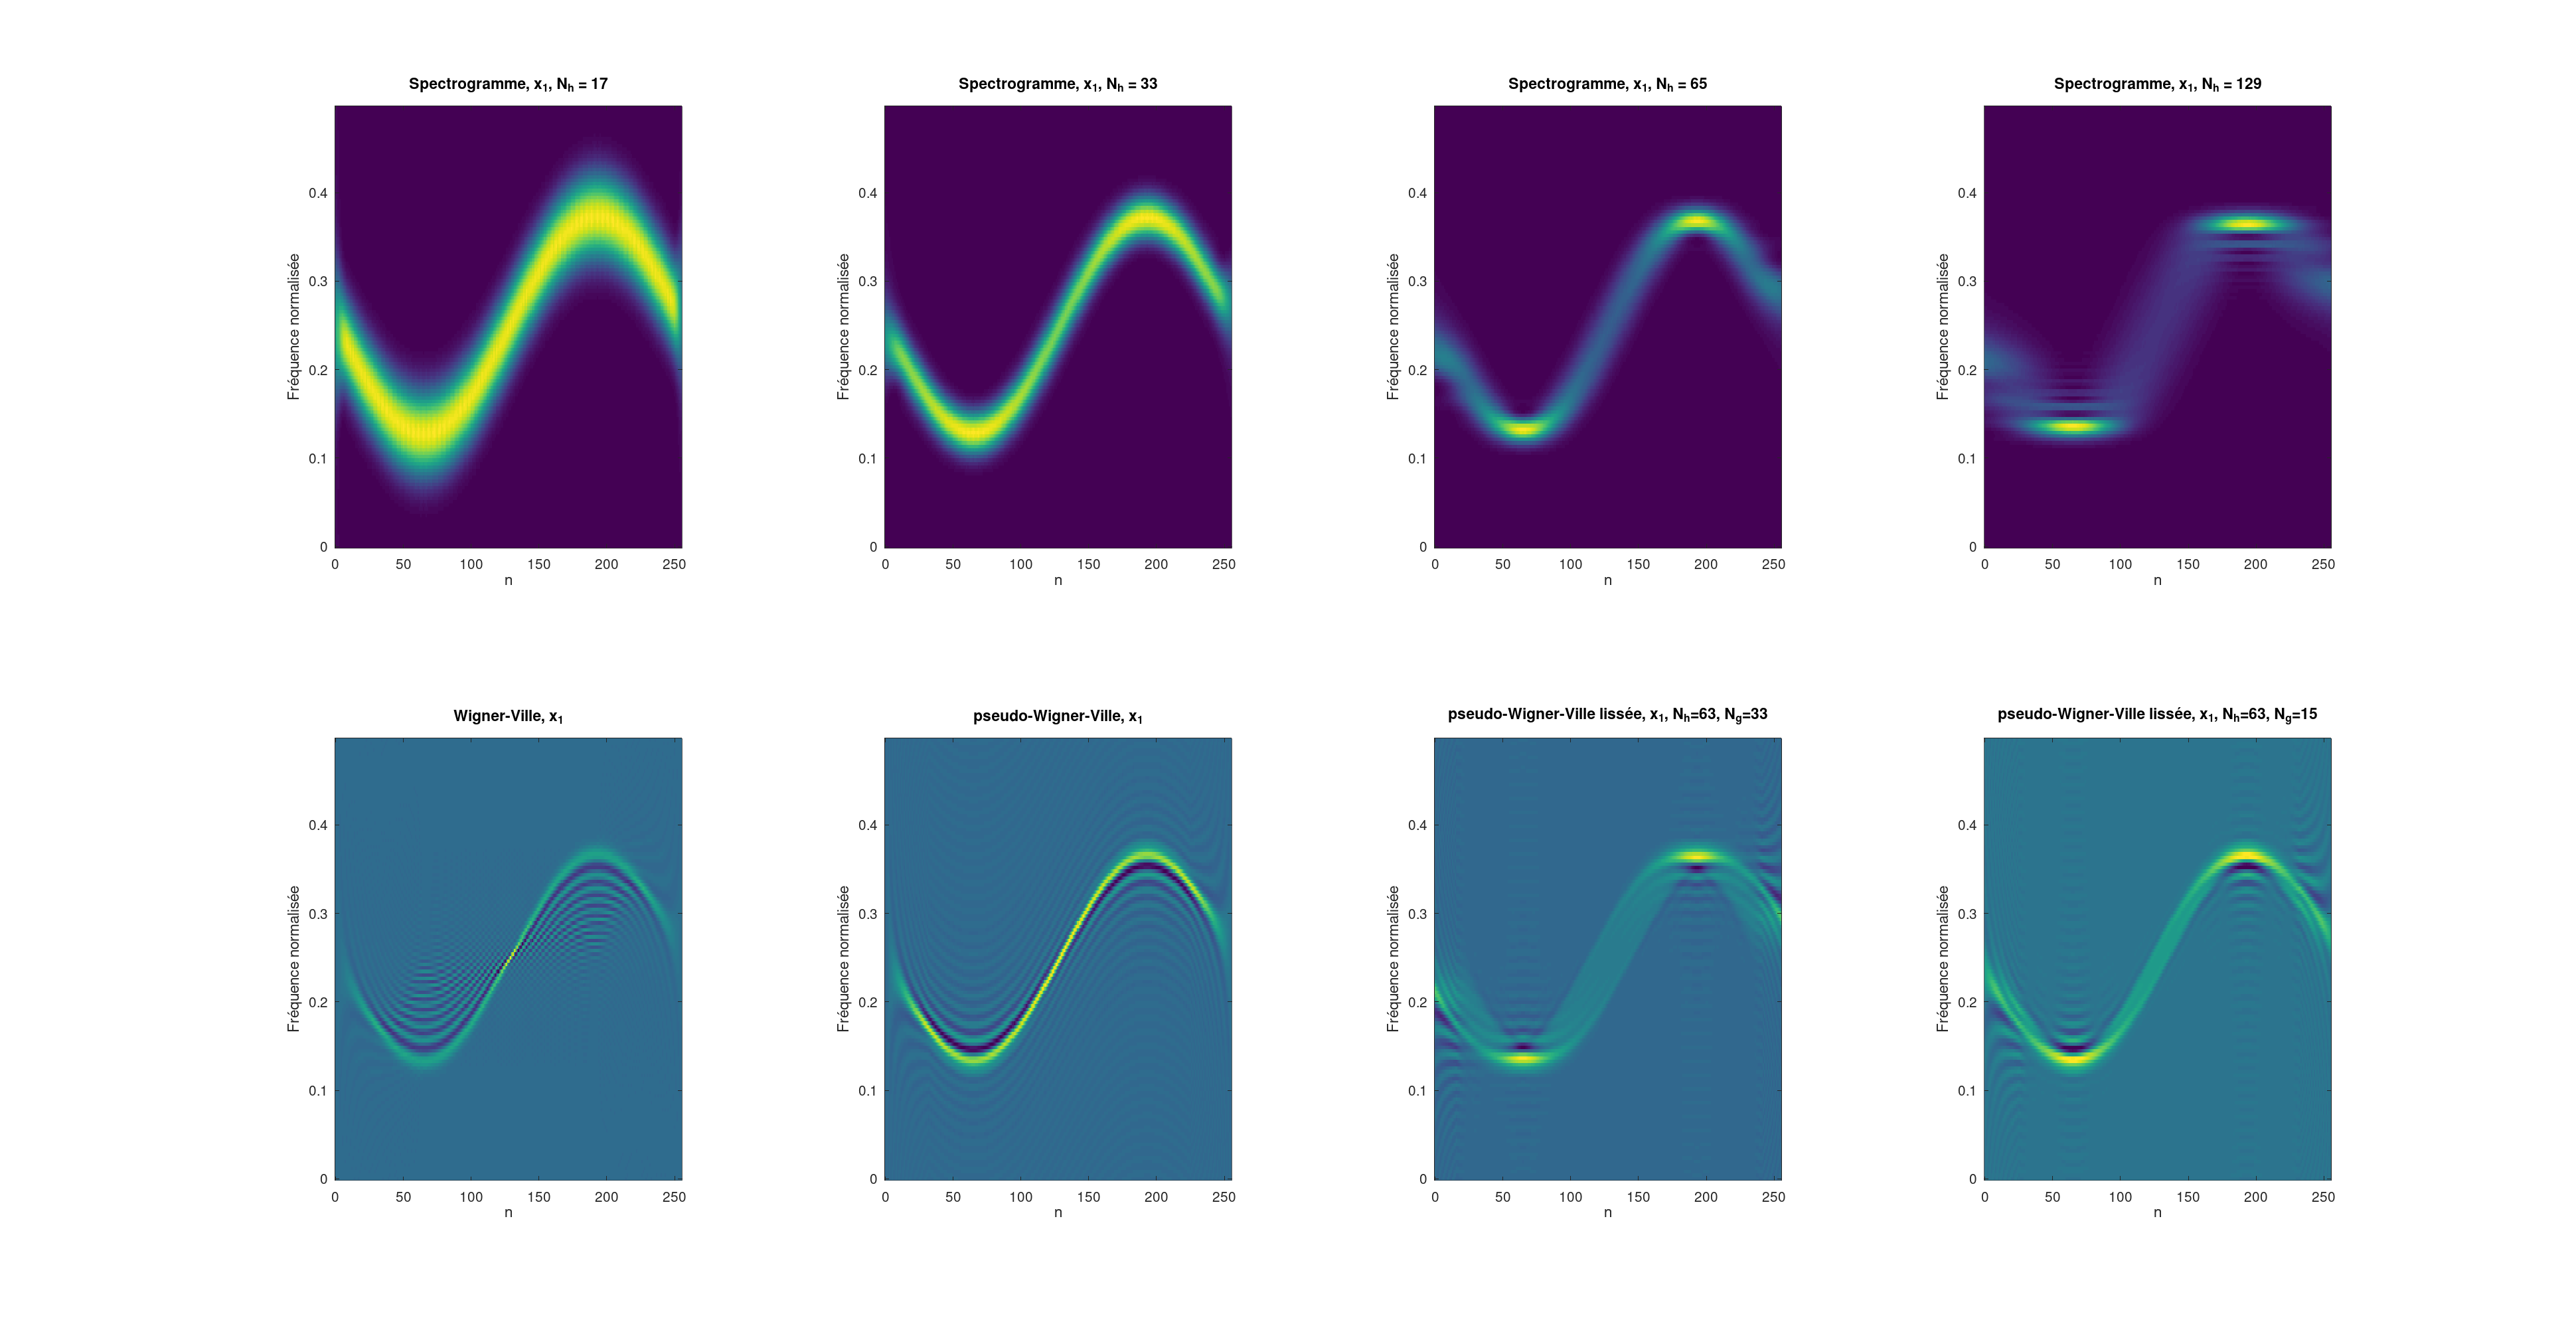
\includegraphics[width=\textwidth]{repr1}
    \centering
\end{figure}

\begin{figure}[H]
    \caption{Tracés $x_2$}
    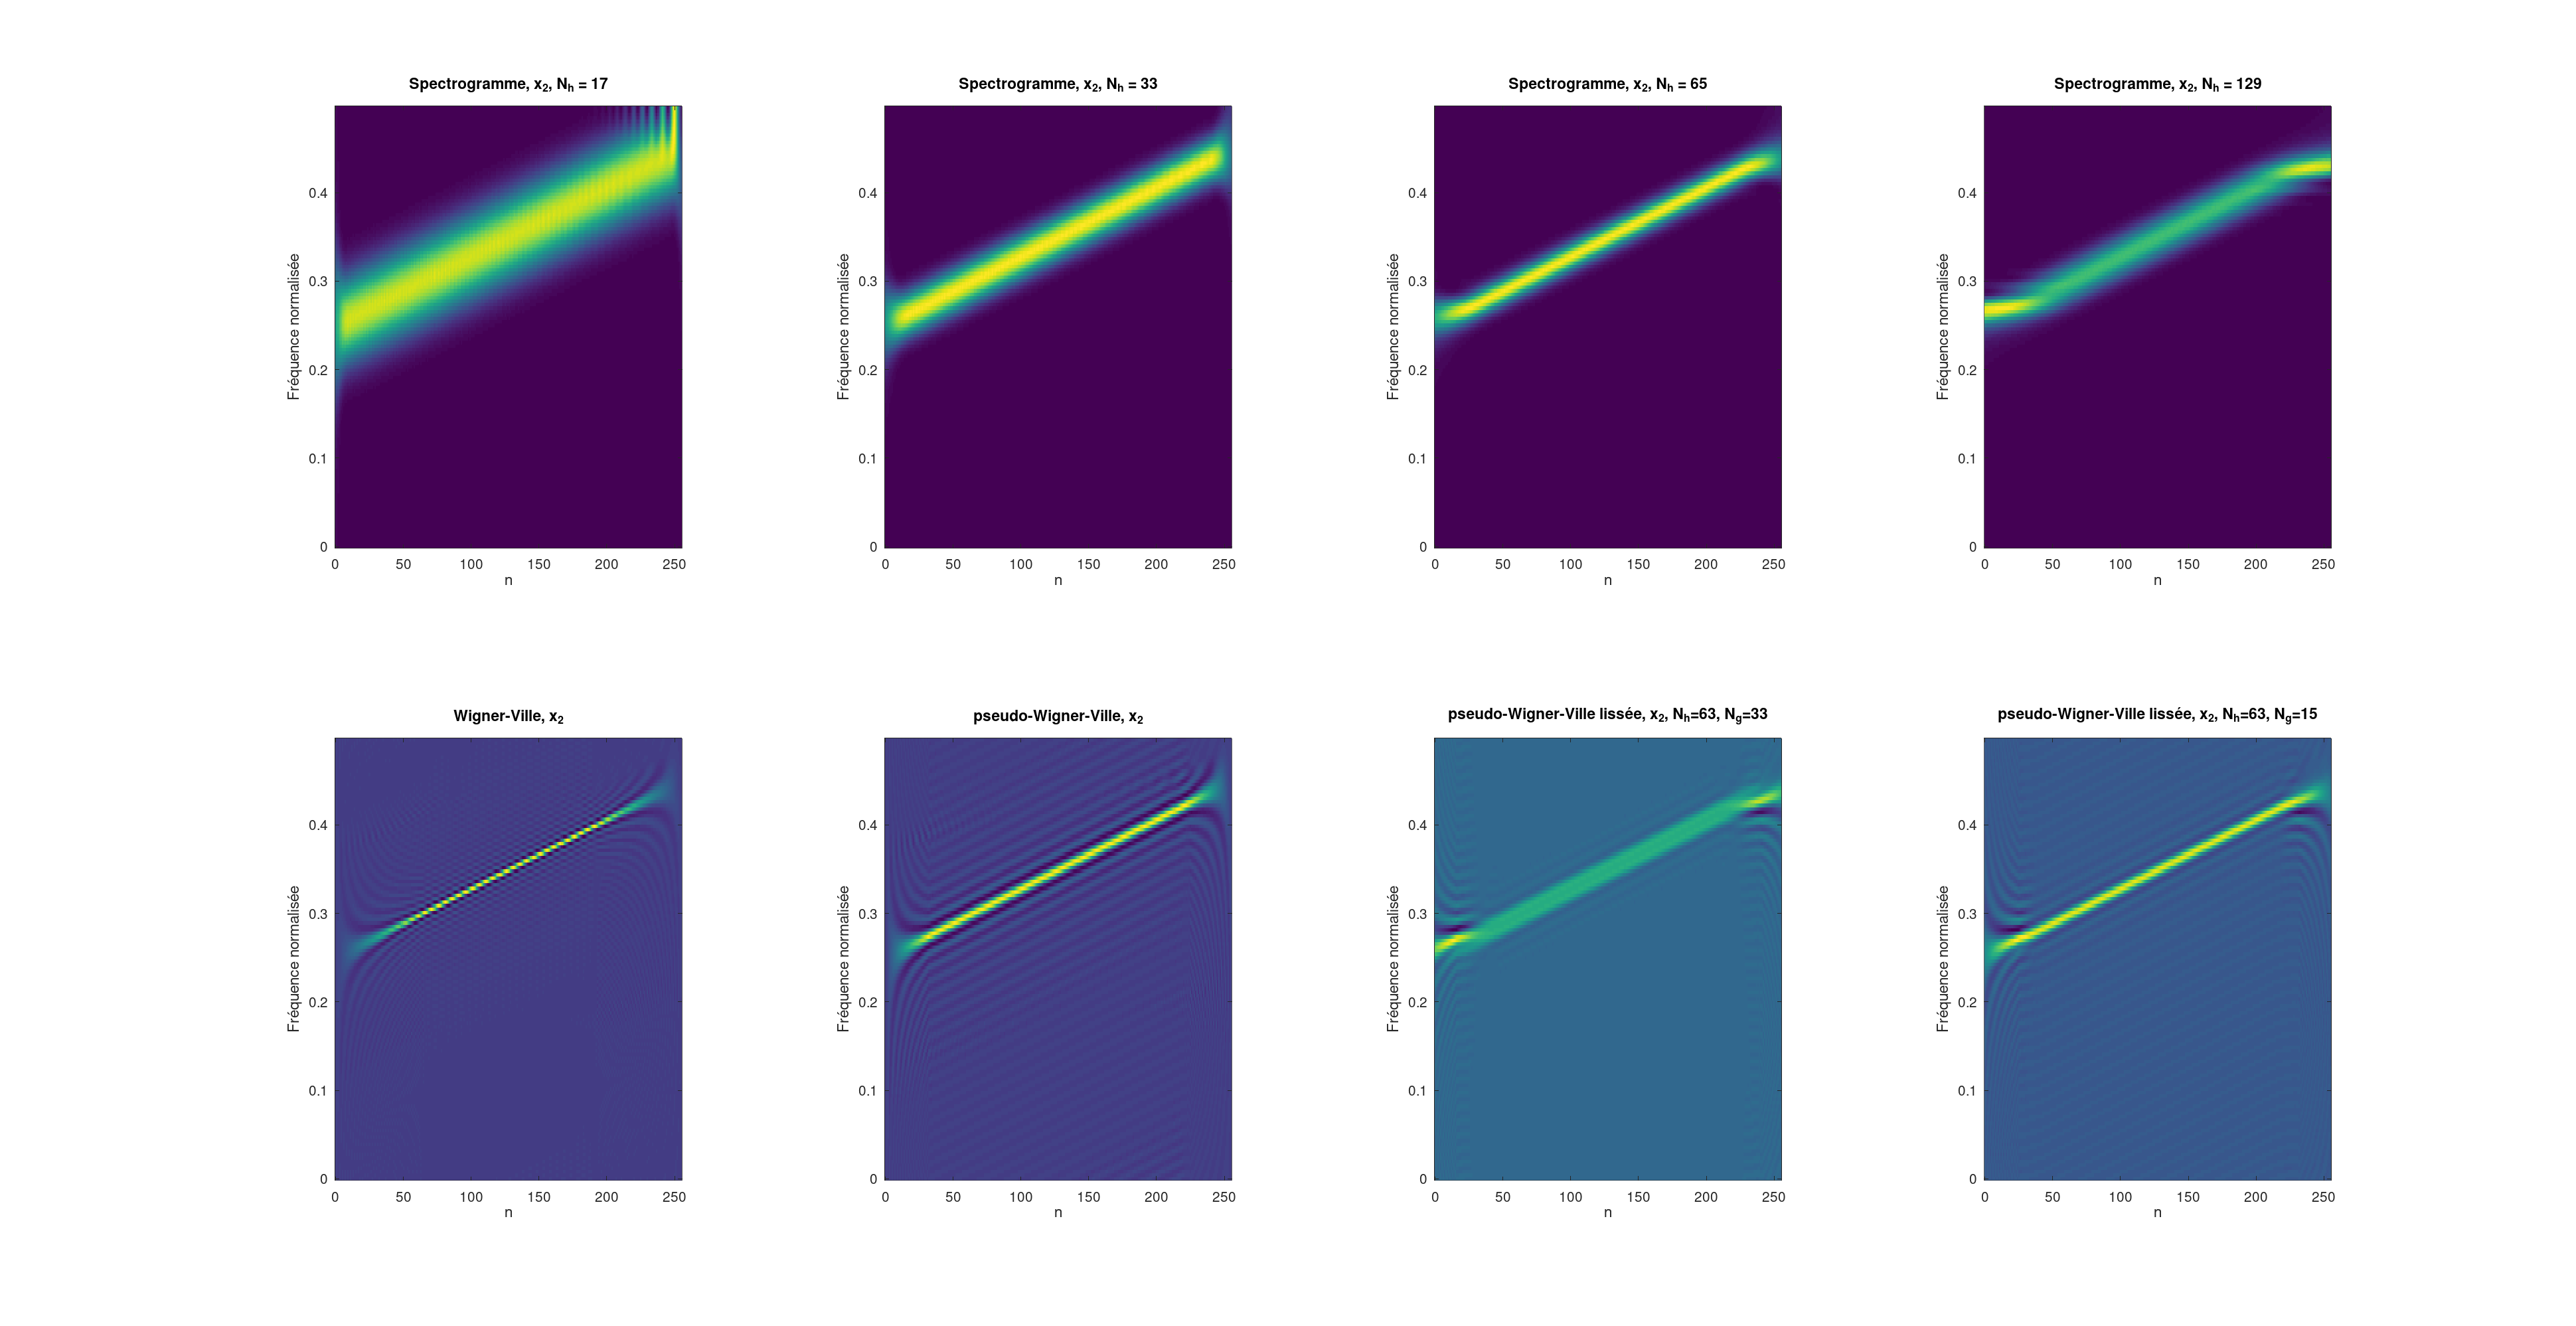
\includegraphics[width=\textwidth]{repr2}
    \centering
\end{figure}

\begin{figure}[H]
    \caption{Tracés $x_3$}
    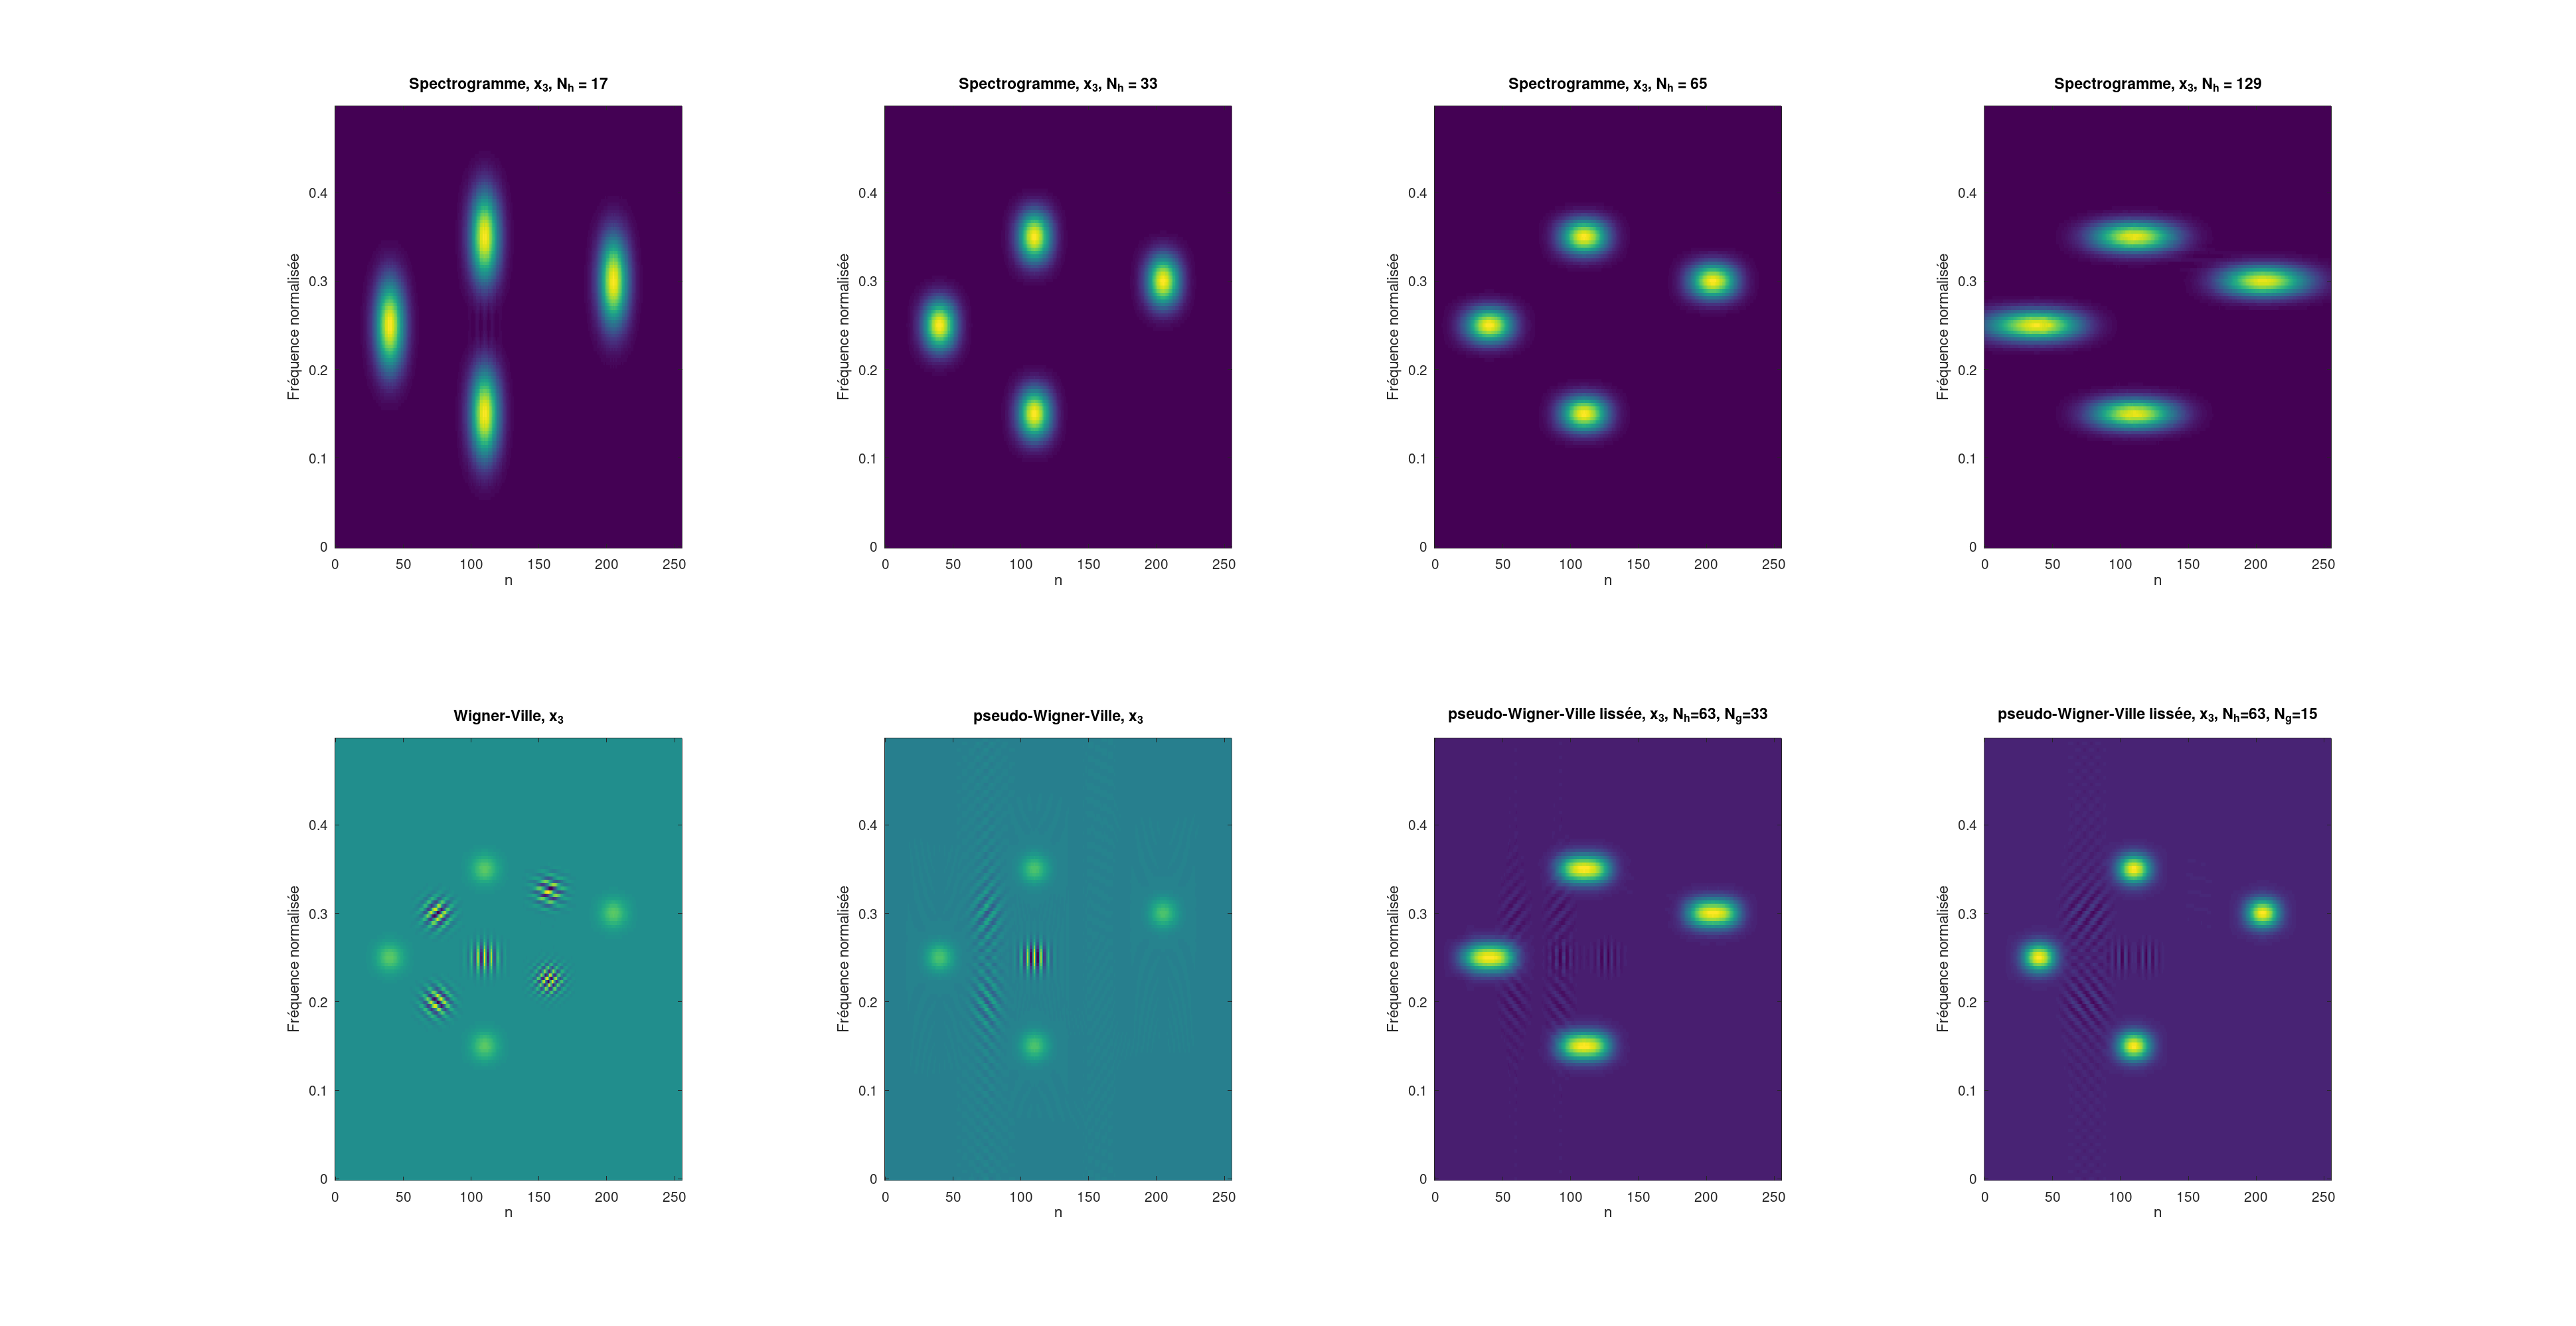
\includegraphics[width=\textwidth]{repr3}
    \centering
\end{figure}

On arrive alors à interpréter facilement les resultats avec ce type de représentation.
\\ En utilisant des fenêtres longues, on a une bonne résolution spectrale mais mauvaise temporelle. Pour les fenêtres courte c'est l'inverse.
La fenêtre de taille moyenne est un bon compromis.

\subsection{Influence du bruit}

Perturbons les signaux à l'aide d'un bruit additif gaussien pour un rapport signal sur bruit de
10dB, on obtient les allures temporelles suivantes :

\begin{figure}[H]
    \caption{Allure temporelles des signaux bruités}
    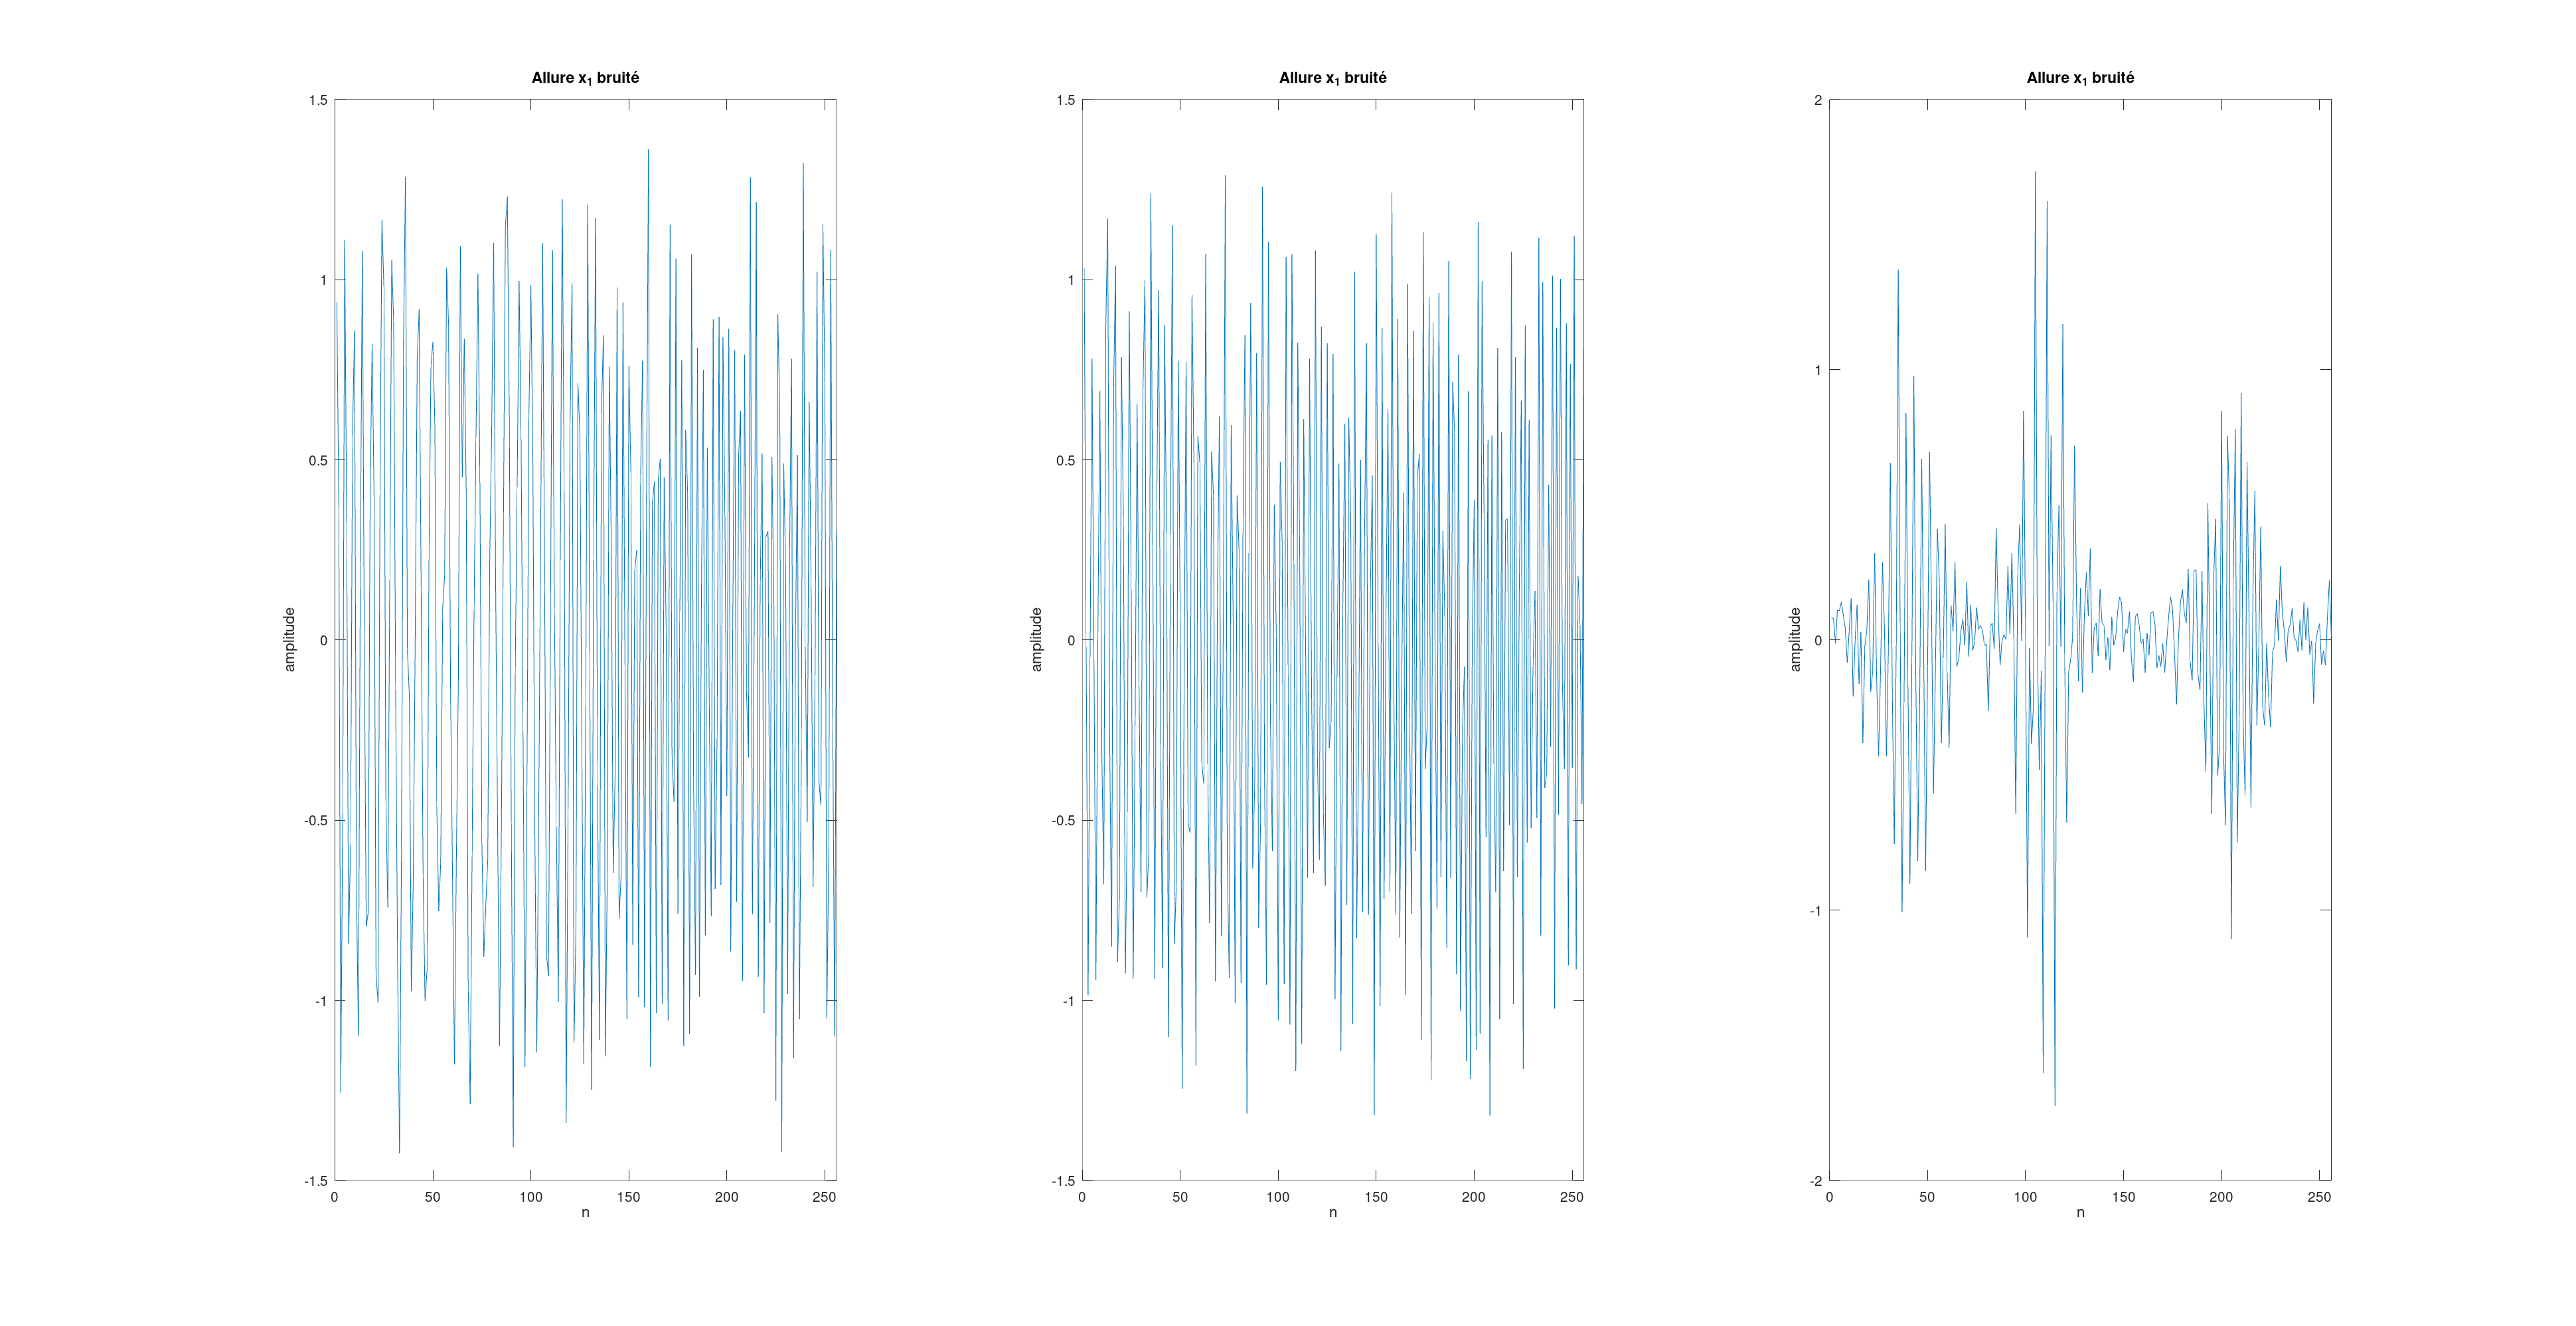
\includegraphics[width=\textwidth]{bruit}
    \centering
\end{figure}

Les différentes représentations suivantes deviennent alors (avec $x_4$ correspondant à $x_1$ bruité,
$x_5$ à $x_2$ bruité et $x_6$ à $x_3$ bruité) :

\begin{figure}[H]
    \caption{Tracés $x_1$ bruité}
    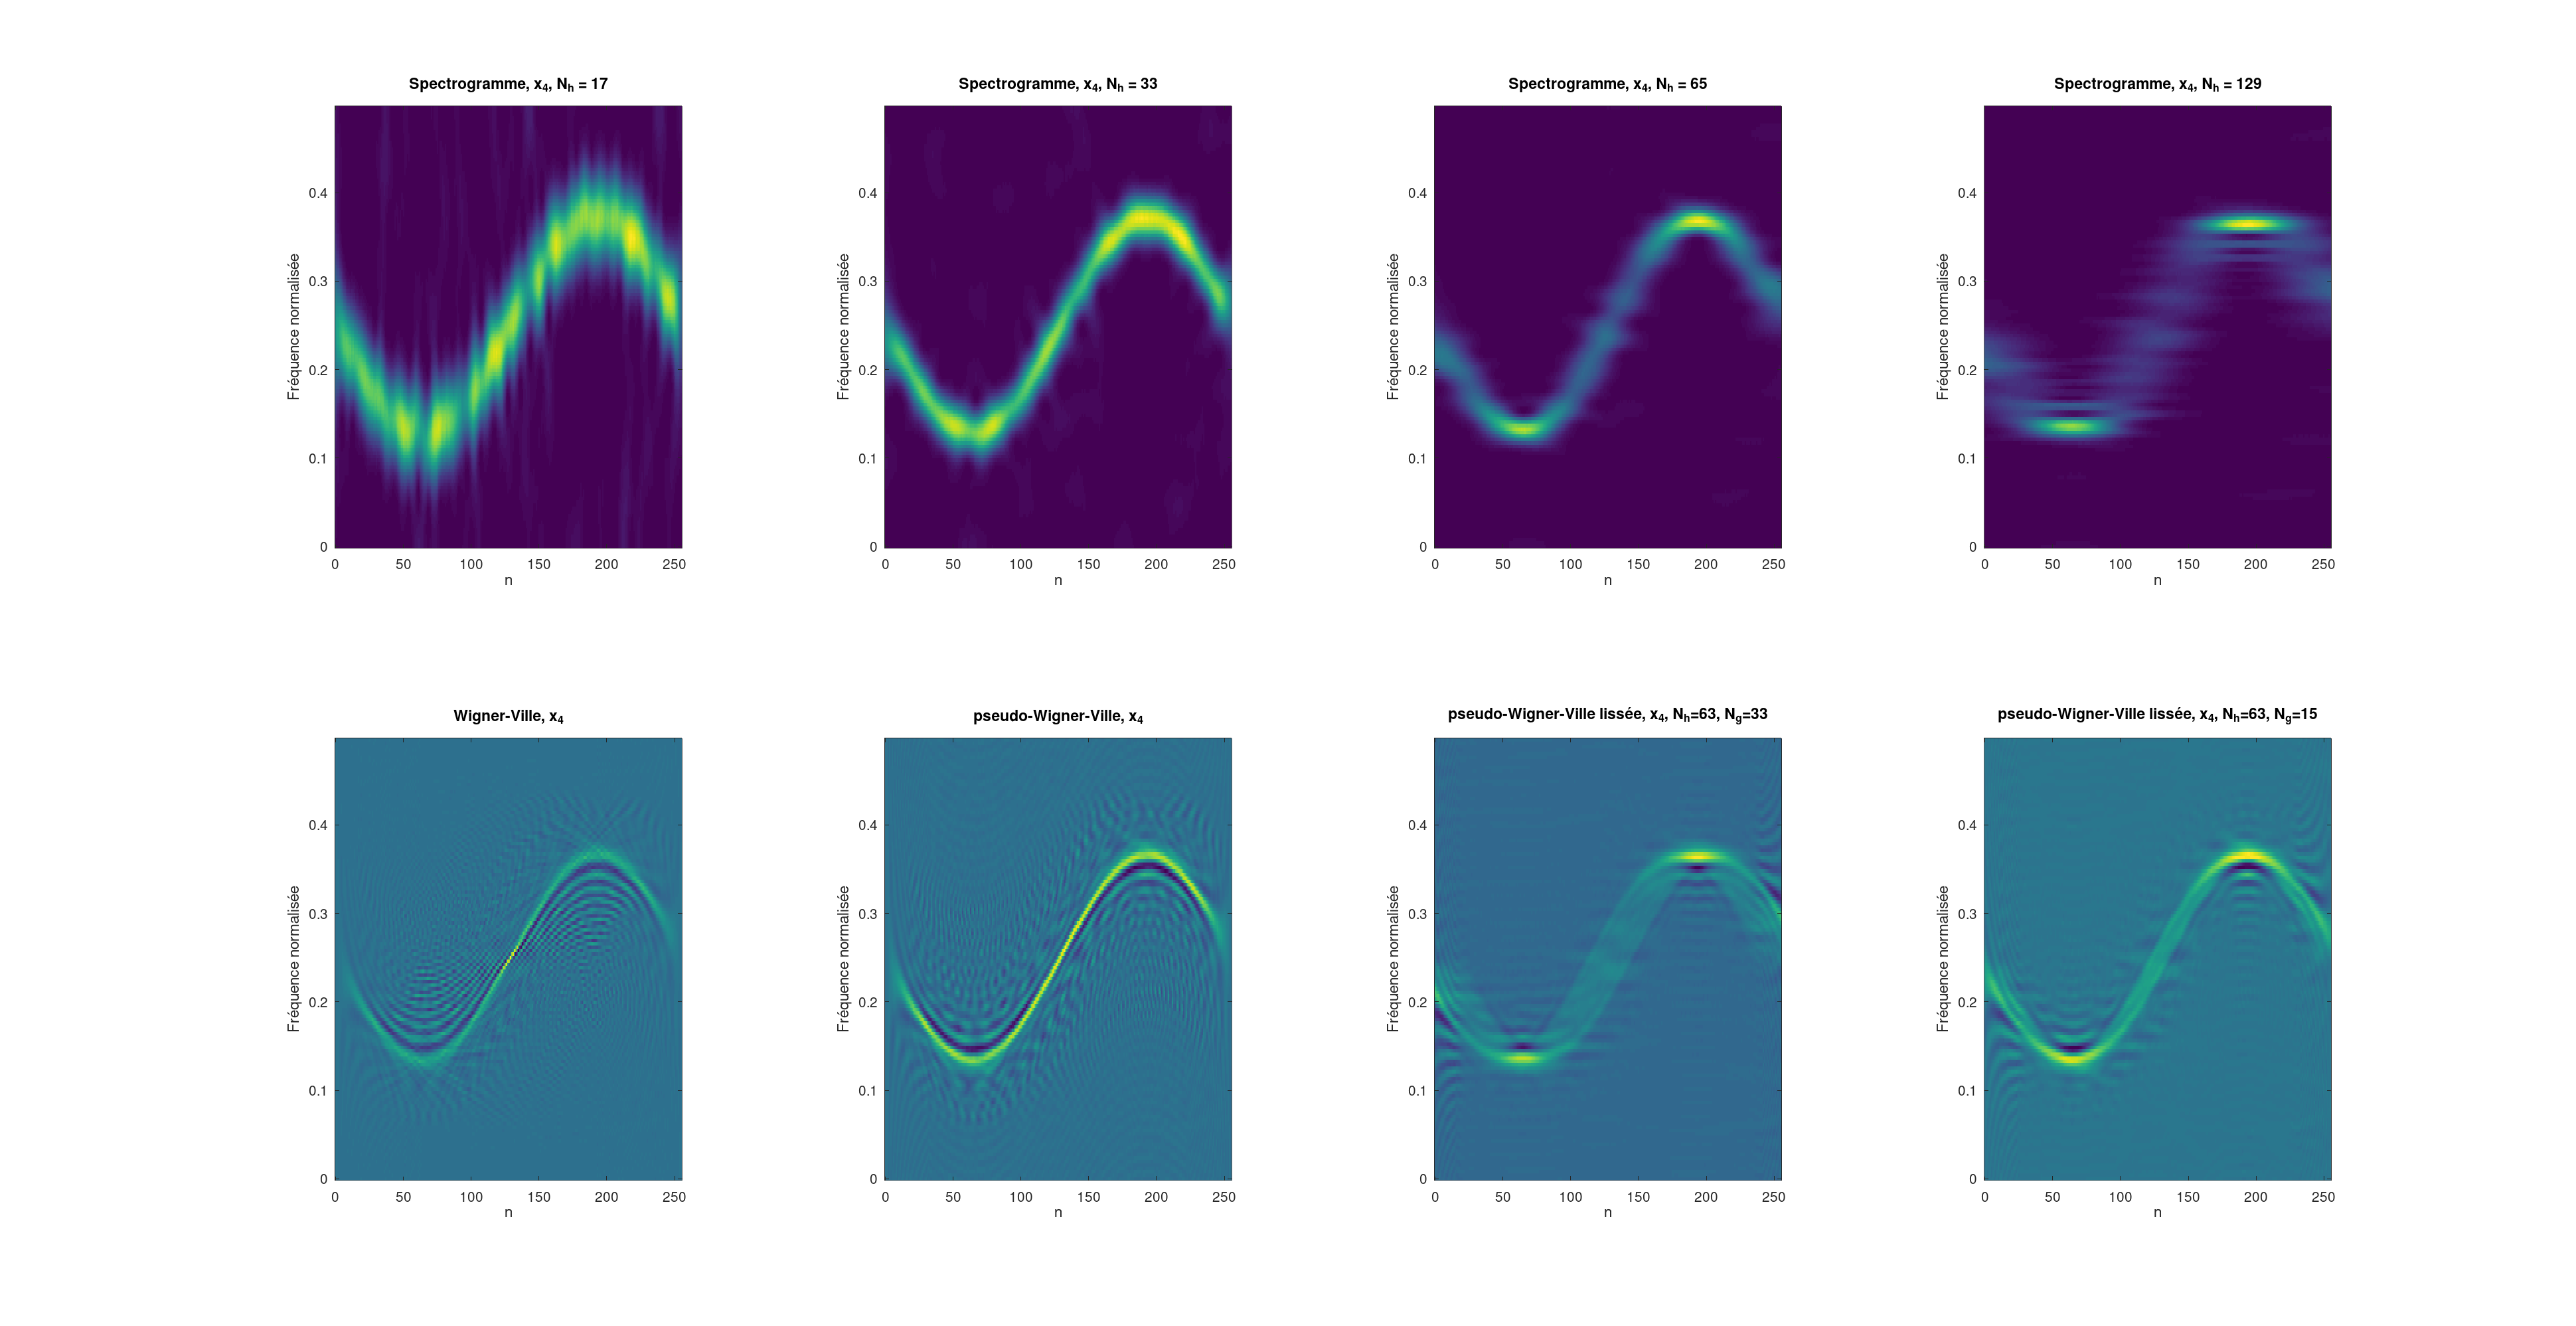
\includegraphics[width=\textwidth]{repr4}
    \centering
\end{figure}

\begin{figure}[H]
    \caption{Tracés $x_2$ bruité}
    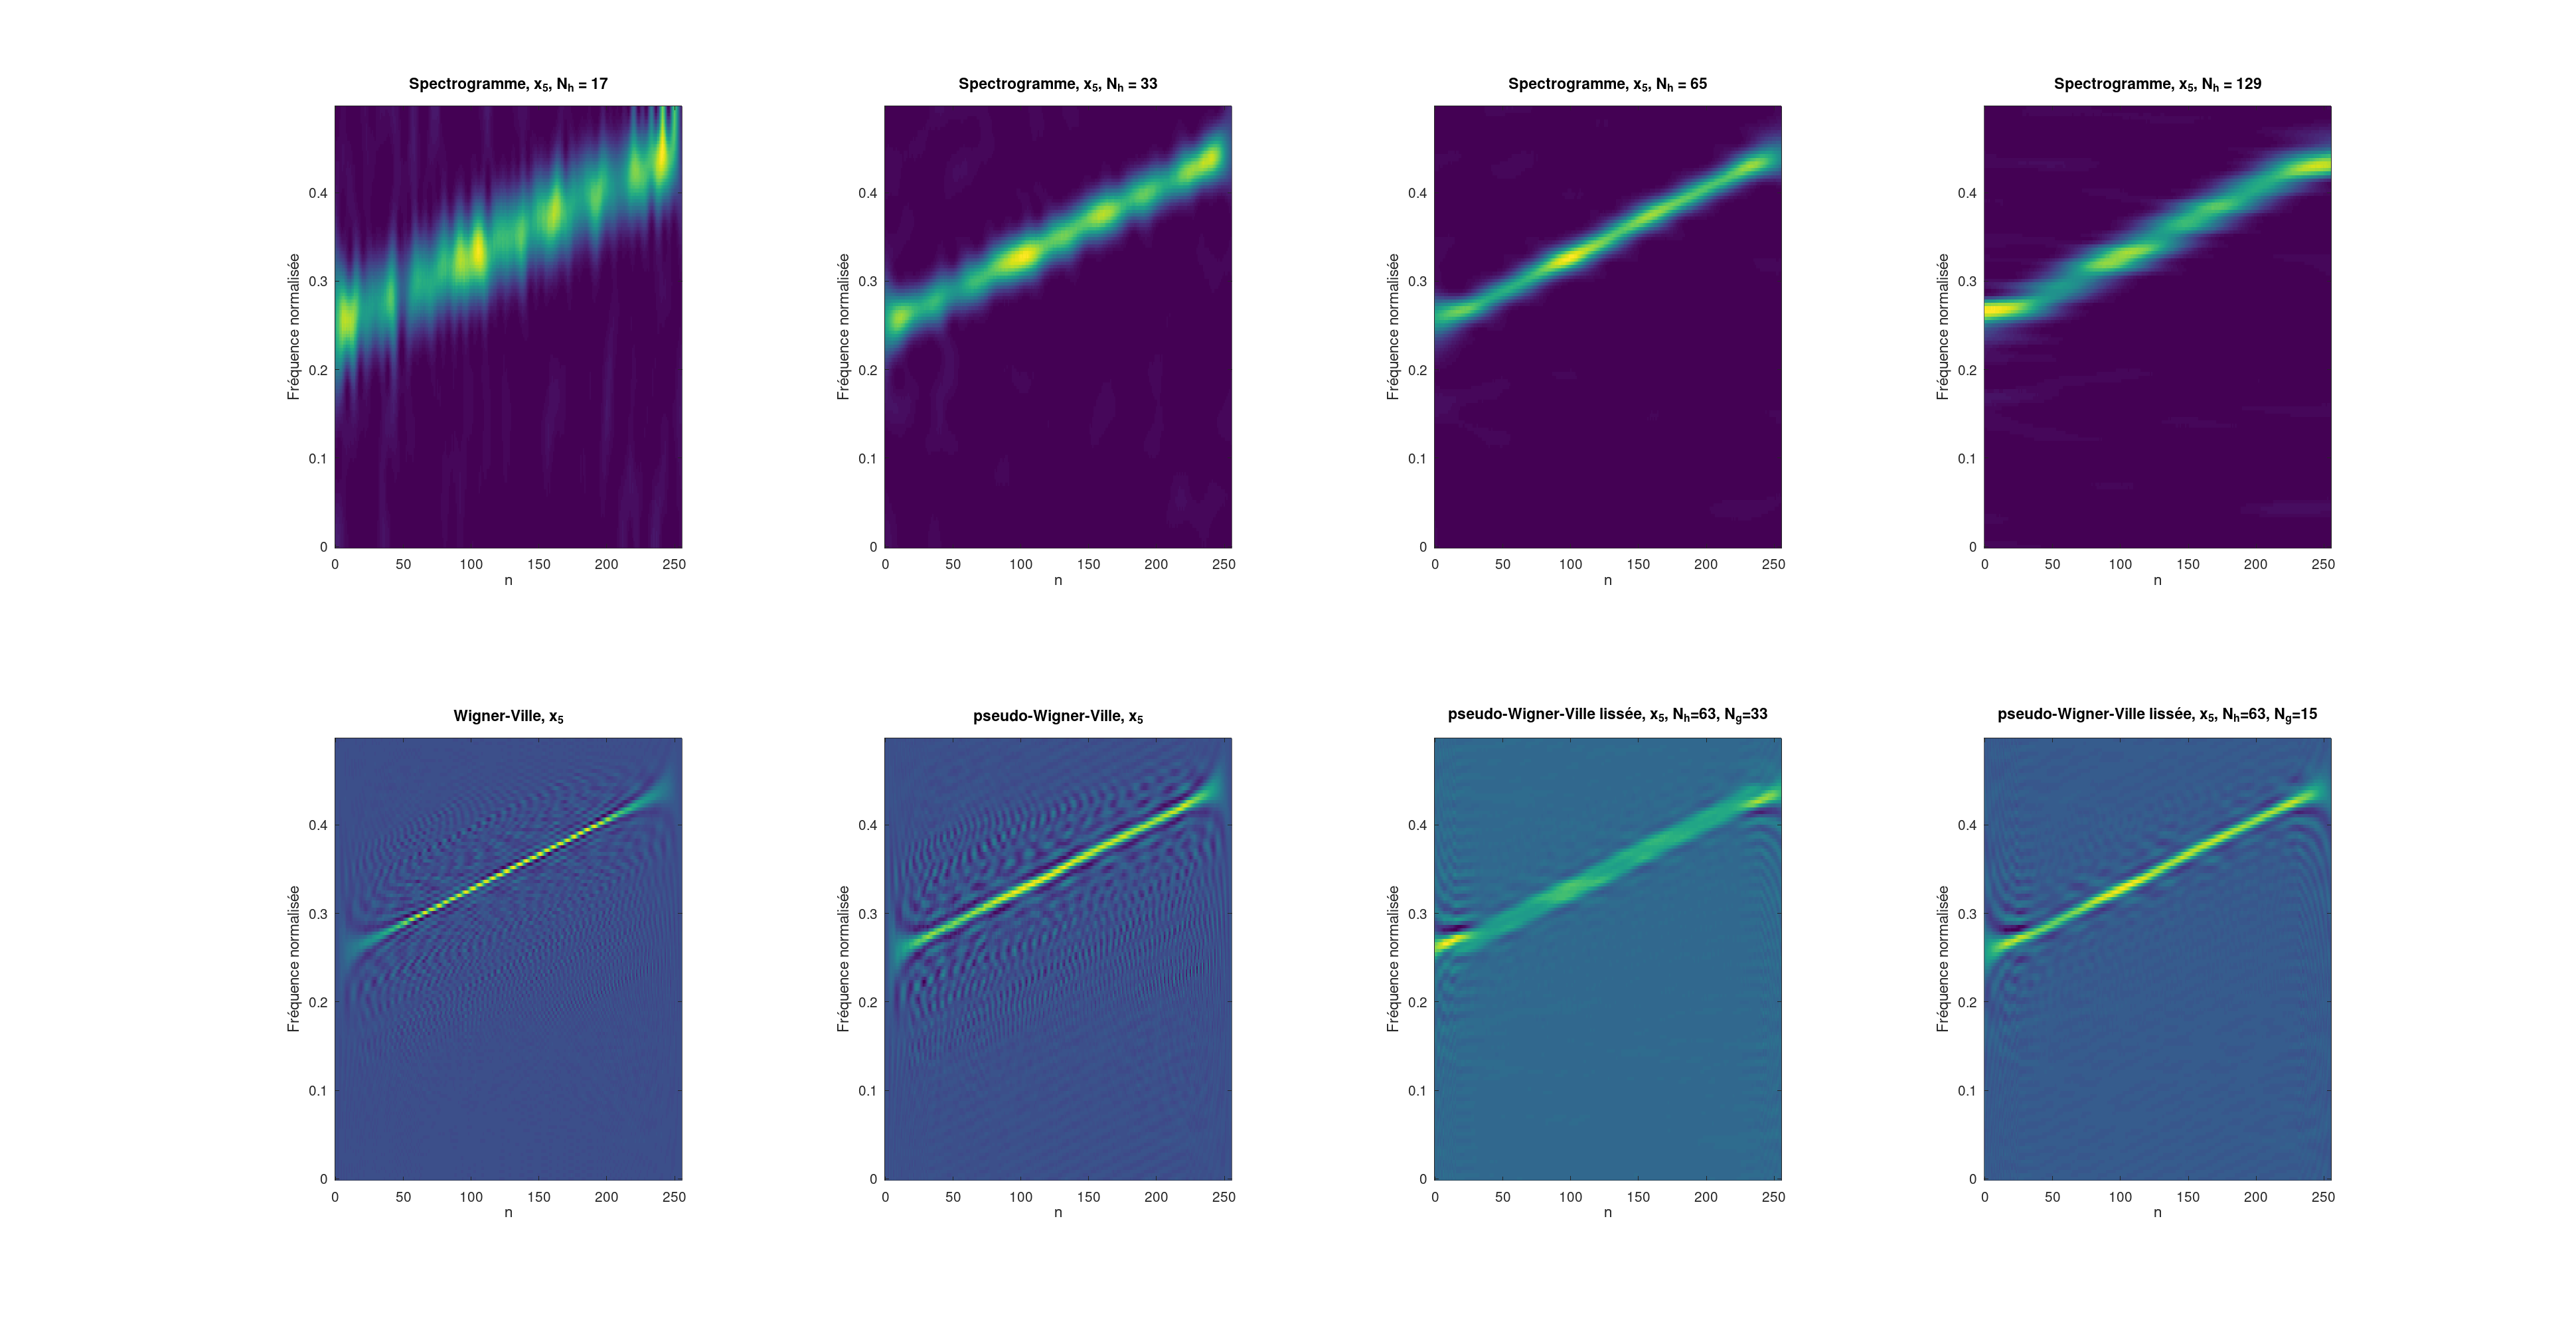
\includegraphics[width=\textwidth]{repr5}
    \centering
\end{figure}

\begin{figure}[H]
    \caption{Tracés $x_3$ bruité}
    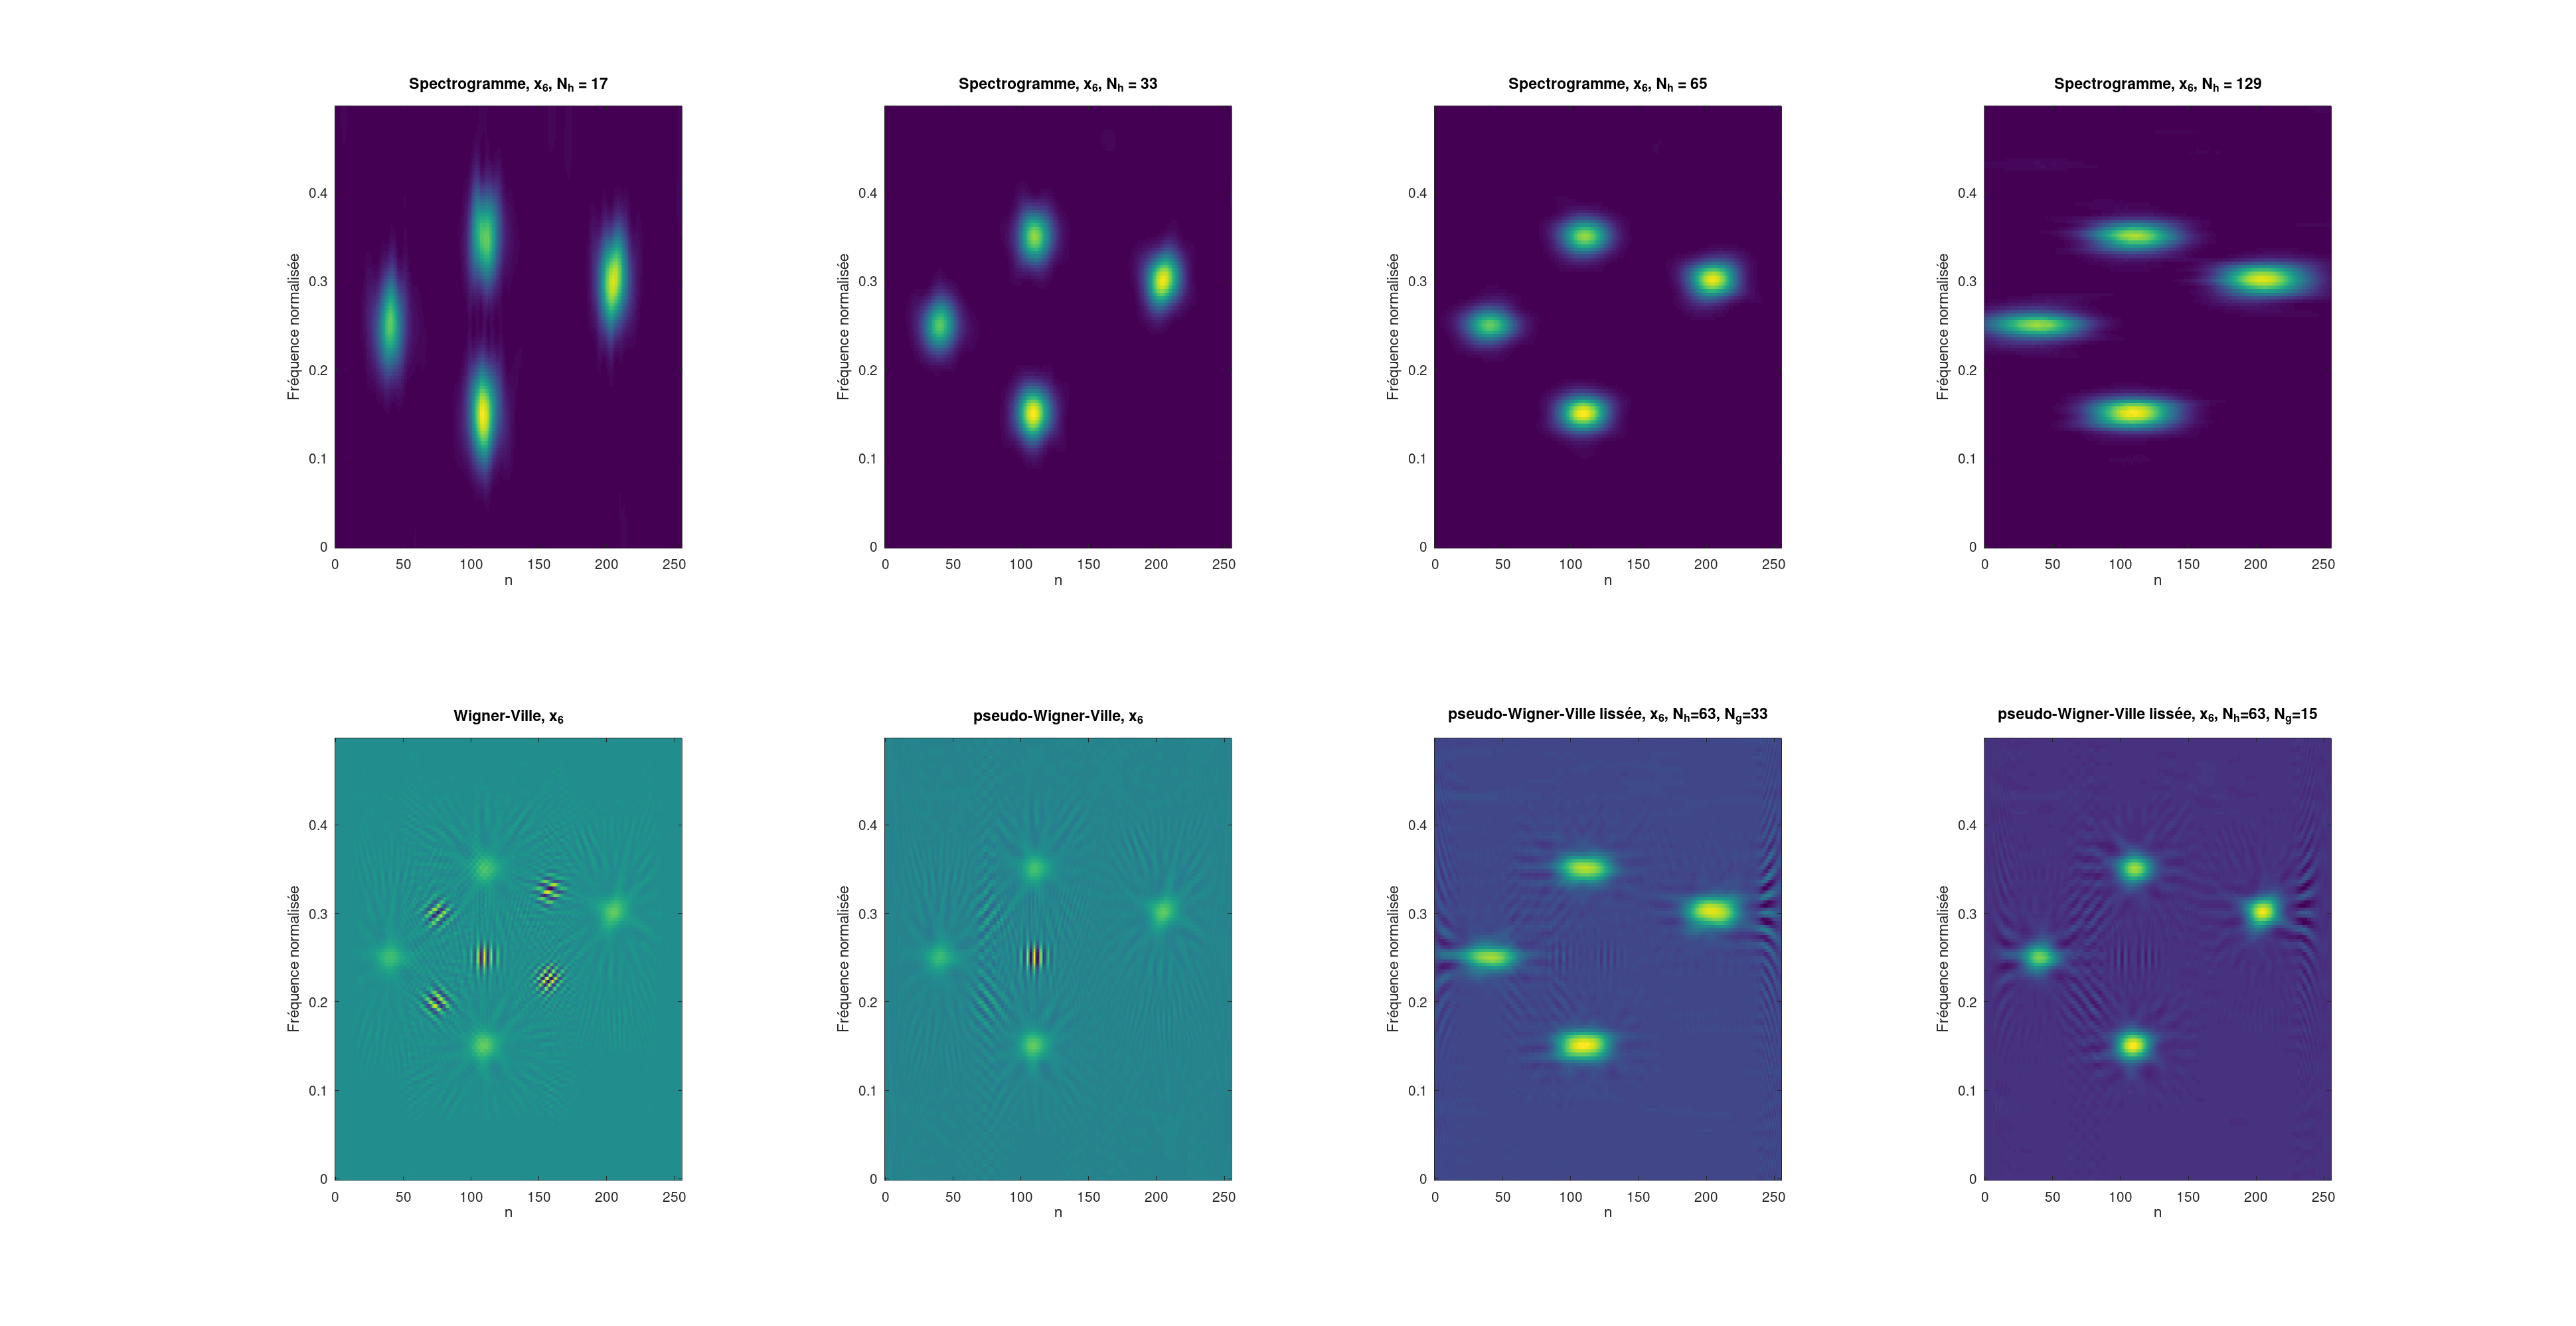
\includegraphics[width=\textwidth]{repr6}
    \centering
\end{figure}

On remarque que les problèmes de résolutions des petites fenêtres et grande fenêtres sont amplifiées par le bruit.
\pagebreak

\section{Détection et reconstruction d'une partition musicale}

\begin{enumerate}

    \item{On charge le fichier à l'aide de la fonction \texttt{audioread} de matlab}

    \item{Représentons l'allure temporelle et le spectrogramme en échelle logarithmique de ce signal :
	\begin{figure}[H]
   		\caption{Allure temporelle et spectrogramme }
        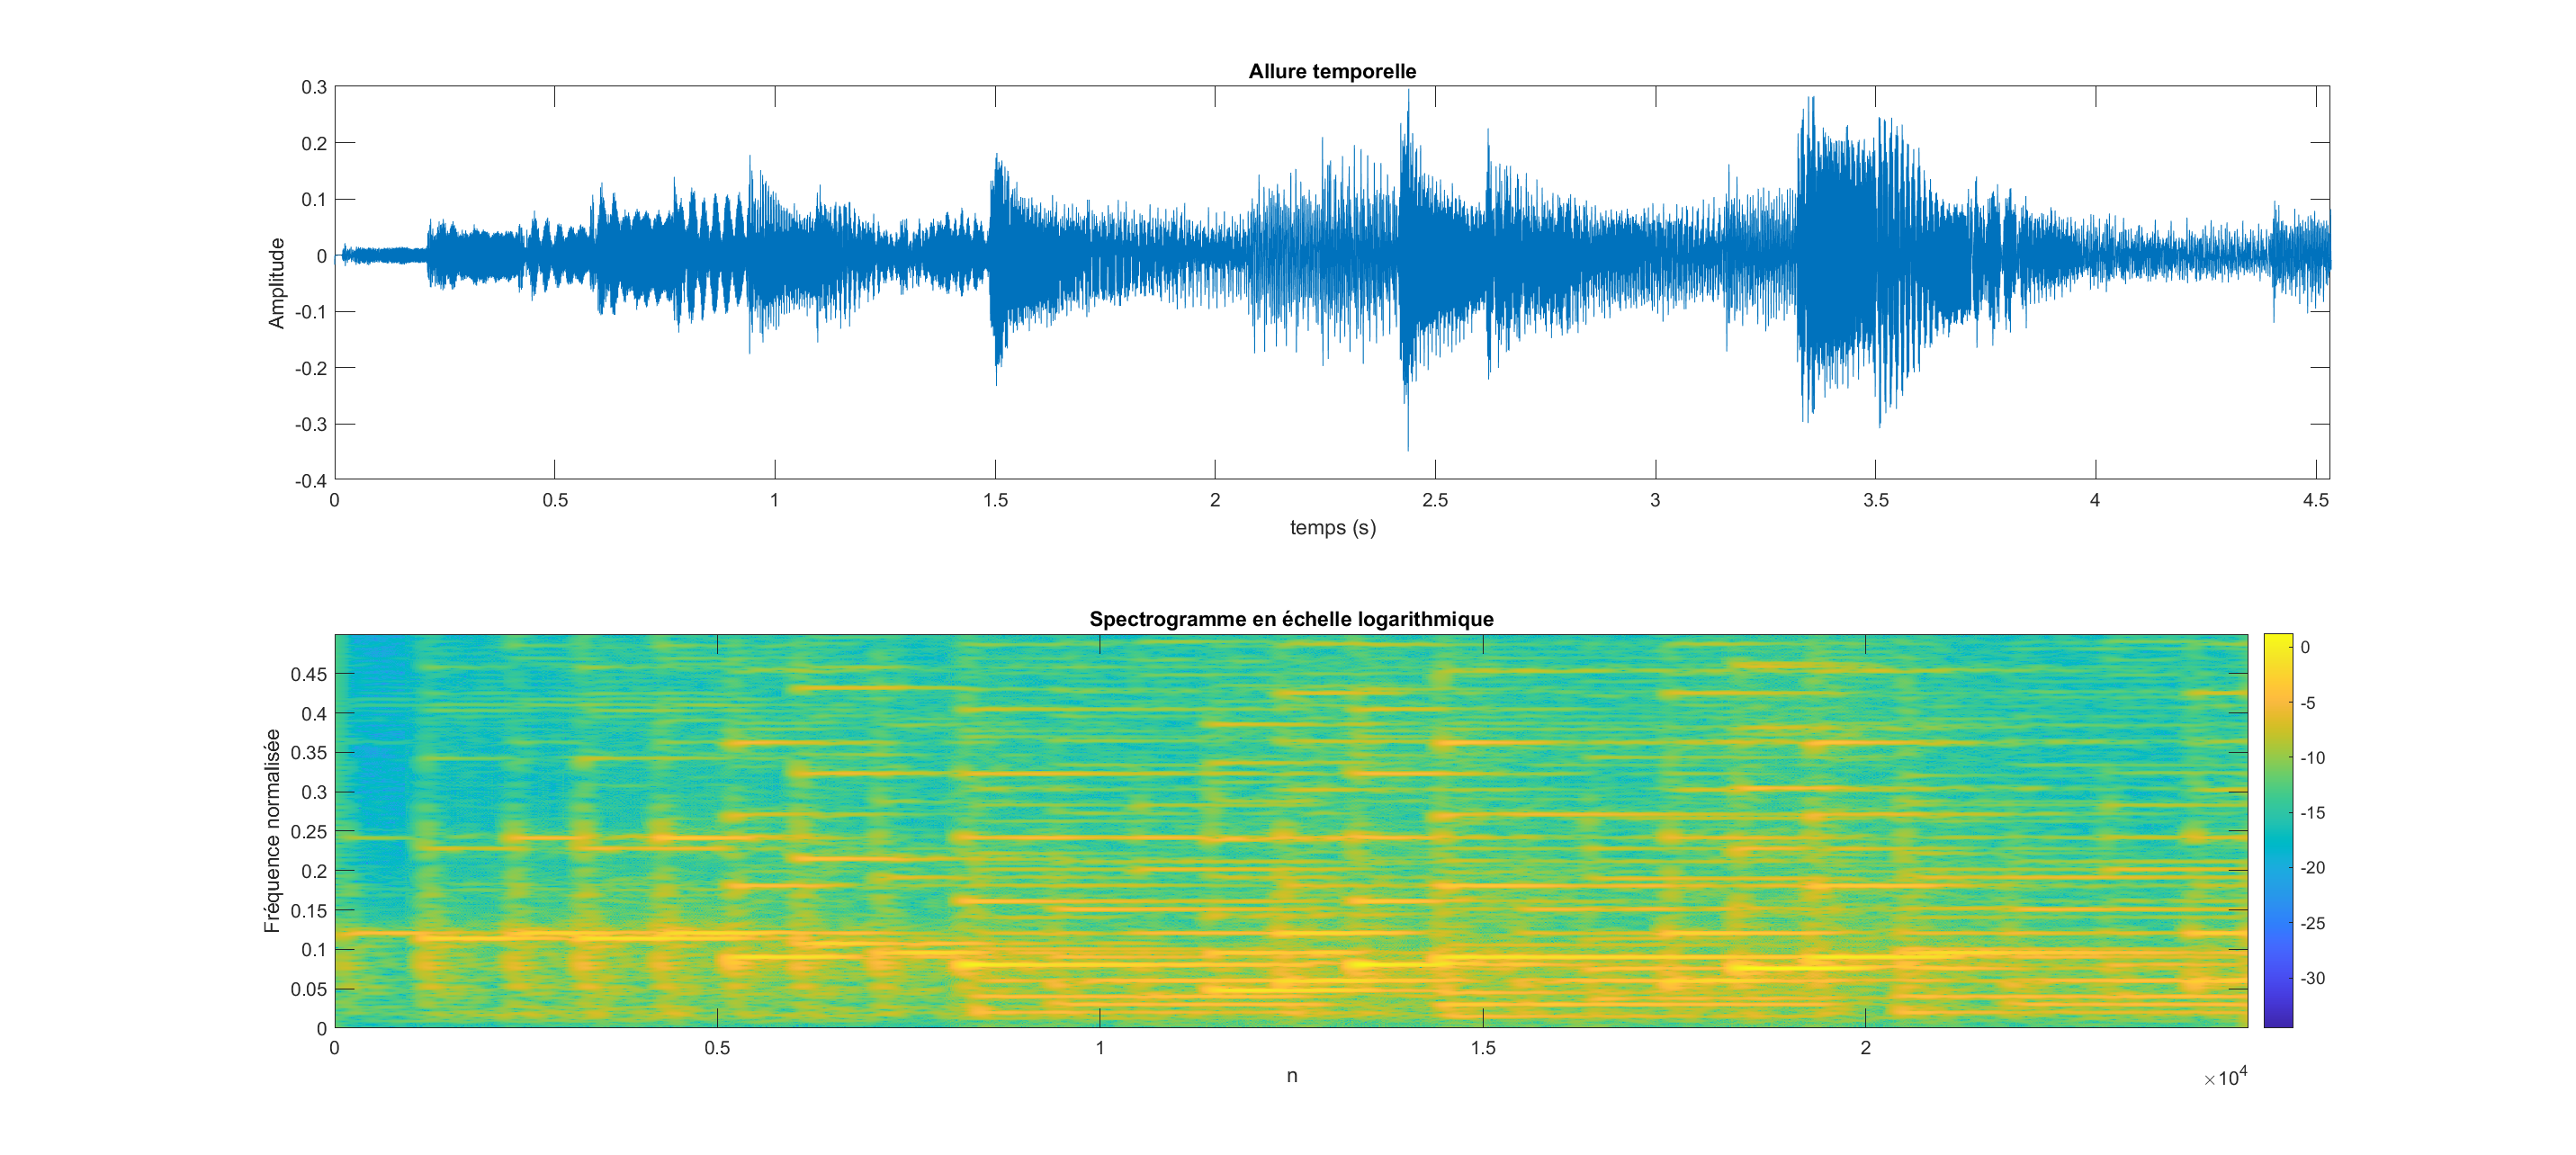
\includegraphics[width=\textwidth]{ex2}
        \centering
    \end{figure}
        }

    \item{On peut ensuite calculer pour un temps tau la différence du contenue frequentiel entre tau et tau +1 en mesurant un indice de stationnarité.}

    \item{Une grande différence entre tau et tau+1 marque alors le passage d'une note à une autre. On peut alors trouver les maximas de notre fonctions I qui prenais la différence du contenue fréquentiel en ordonnées pour un temps t en abscisse. On cherche donc à savoir quand cette fonction est maximale pour détecter ses changements de fréquences }

    \item{On obtient alors une liste d'instant sur laquelle on va itérer. Pour chacun de ces instants, on calcule la fréquence pour laquelle la transformée de fourrier est maximale en module. On trouve alors une fréquence pour laquelle on cherche à associer une note}
    
    \item{On obtient alors la liste de notes suivante :
    \begin{figure}[H]
    	\caption{Liste de notes obtenues}
    	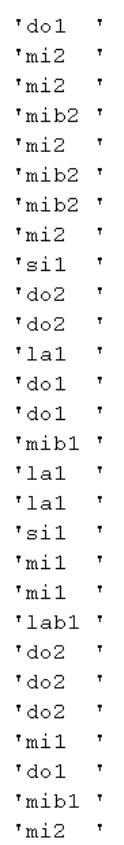
\includegraphics[width=0.1\textwidth]{notes}
        \centering
    \end{figure}}
    
\item{On peut finalement, envoyer cette liste de note ainsi que le temps préalablement calculé de chaque note à une fonction \texttt{genere\_morceau} pour reconstituer notre mélodie.}

\end{enumerate}

\begin{appendices}

    \section{Scripts Représentation temps-fréquence de signaux simulés}

    \lstinputlisting[language=Matlab]{../ex1.m}

    \section{Scripts Détection et reconstruction d'une partition musicale}

    \lstinputlisting[language=Matlab]{../ex2.m}

\end{appendices}

\end{document}
